\chapter{Metodología}\label{cap4:Metodologia}

\section{Metodología}

\begin{figure}[H]
    \centering
       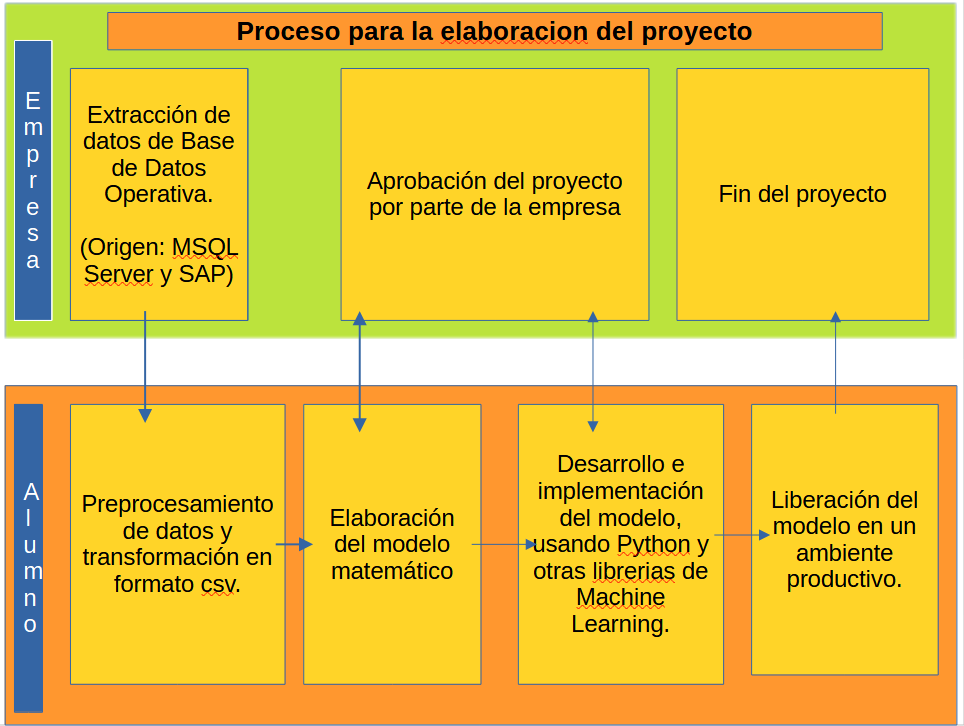
\includegraphics[width=12cm, height=7cm ]{Imagenes/Proceso_Proyecto.PNG }
      \caption{Metodología}
      \label{fig:meto}
\end{figure}

La metodología para realizar el proyecto se explica con la figura anterior.

\begin{itemize}
    \item La empresa proporciona la información con la que quiere que se desarrolle el modelo en formato Excel. \medskip
    \item Se recibe el archivo Excel y se realiza la limpieza y preprocesamiento de datos y se convierte a un formato de texto CSV , para usarlo como entrada por el algoritmo de aprendizaje . \medskip
    \item Se elabora el modelo y se interactúa con la empresa , hasta lograr un modelo este de acuerdo a sus necesidades. \medskip
    \item Una vez aprobado el modelo, se desarrolla el algoritmo usando el lenguaje de programación Python y otras librerías adicionales.\medskip
    \item El script o programa es evaluado por la empresa, la cual da su aprobación en cuanto a la funcionalidad requerida. \medskip
    \item Completado el anterior paso la empresa da su aprobación, con lo cual queda concluido el proyecto terminal. \medskip 
\end{itemize}

Una parte de dataset de trabajo es el siguiente :

\begin{figure}[H]
    \centering
       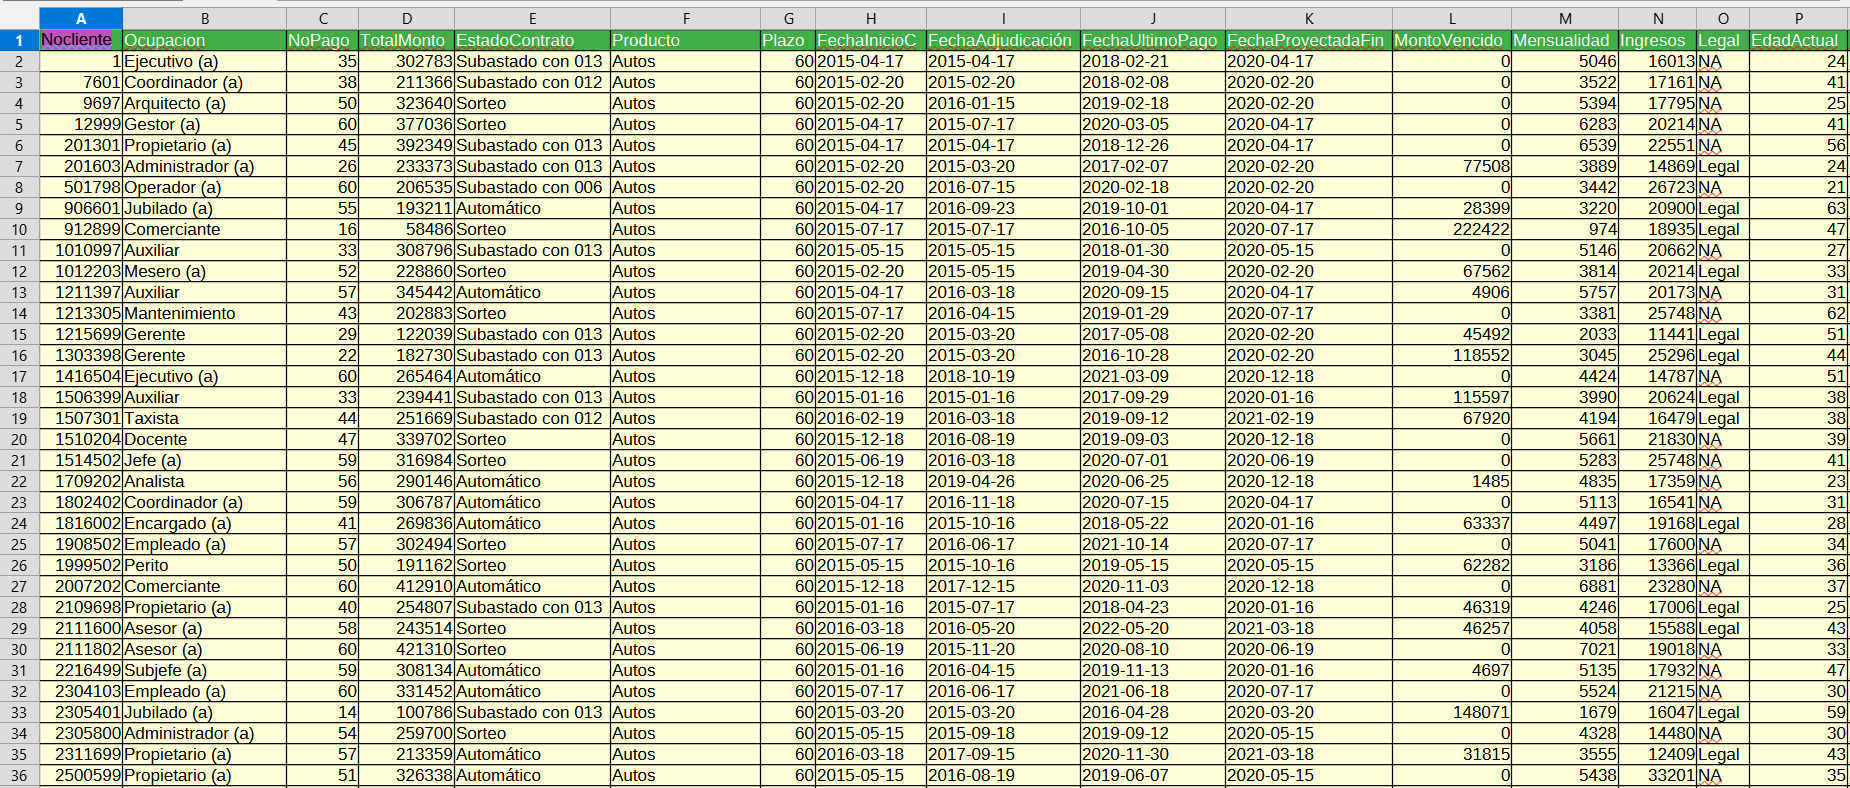
\includegraphics[width=16cm, height=10cm ]{Imagenes/Datos_Clientes1.PNG }
      \caption{Datos de los clientes (Bloque 1)}
      \label{fig:clis1}
\end{figure}
\newpage
\begin{figure}[H]
    \centering
       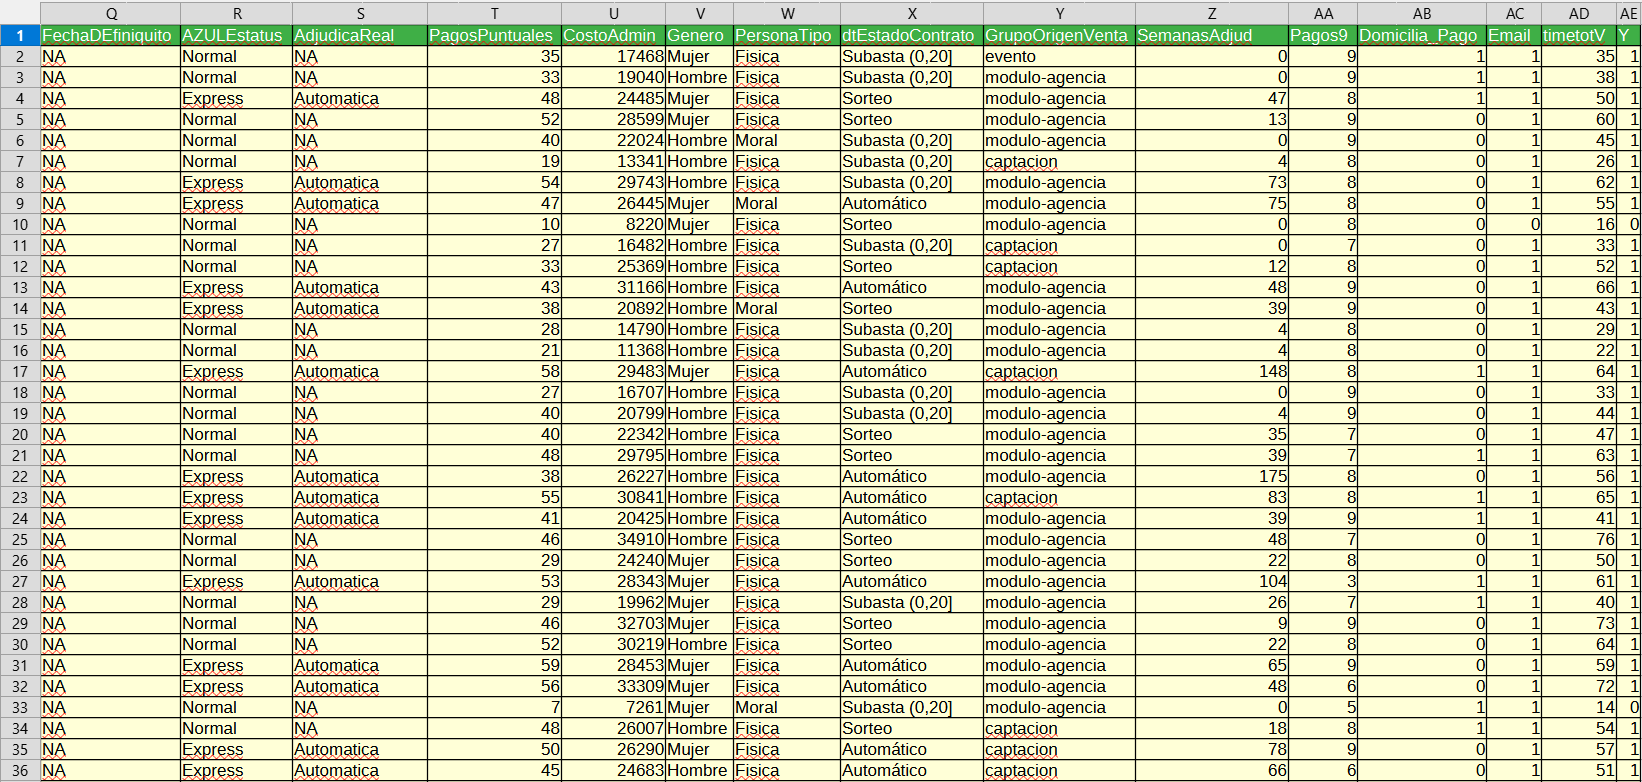
\includegraphics[width=16cm, height=10cm ]{Imagenes/Datos_Clientes2.PNG }
      \caption{Datos de los clientes (Bloque 2)}
      \label{fig:clis2}
\end{figure}
 
\section{Limpieza del dataset}

La limpieza de datos es una etapa esencial en el proceso de machine learning porque garantiza 
que el modelo trabaje con información de calidad, lo que mejora la precisión de sus resultados. 
Con frecuencia, los datos originales contienen errores, valores faltantes, duplicados o ruido, 
lo cual puede desviar el análisis y llevar a conclusiones equivocadas. Al procesar y limpiar los 
datos, se eliminan estas imperfecciones, ayudando a que el modelo se enfoque en patrones verdaderos
en lugar de anomalías. \medskip

La limpieza también permite identificar y gestionar los valores atípicos o outliers, que pueden 
distorsionar los resultados si no se manejan adecuadamente. Además, durante el proceso de 
limpieza, los datos se estandarizan y normalizan, especialmente cuando las variables presentan 
diferentes escalas o unidades; esto evita sesgos en el entrenamiento del modelo. 




    \subsection{Eliminar columnas que contienen un solo valor} 

    Podemos ver las variables categóricas del dataset con la instrucción \medskip
    \begin{itemize}
    \item datasetT.info()
    \end{itemize}
    \newpage
    Y obtenemos la siguiente información como respuesta
    
    \begin{verbatim}
    RangeIndex: 2000 entries, 0 to 1999 
    Data columns (total 31 columns):
    \end{verbatim}

    \begin{table}[H]
        \centering
        \begin{tabular}{|c|c|c|c|c|}
            \hline
            \rowcolor{softblue} % Fila color azul suave
            \textbf{Num} & \textbf{Columna} & \textbf{Count} & \textbf{Non-Null} & \textbf{Dtype} \\
            \hline
            % \rowcolor{lightgray} % Fila color gris claro
            \hline
            0 &	Nocliente &		2000 &	non-null &	int64  \\
            \hline
            1 &	Ocupacion &		2000 &	non-null &	object \\
            \hline
            2 &  NoPago    &          2000 & non-null &  int64  \\
            \hline
            3 &  TotalMonto  &        2000 & non-null &  int64  \\
            \hline
            4 &  EstadoContrato &     2000 & non-null &  object \\
            \hline
            5 &   Producto  &         2000 & non-null &   object \\
            \hline
            6 &  Plazo     &          2000 & non-null &   int64  \\
            \hline
            7 &  FechaInicioC  &      2000 & non-null &   object \\
            \hline
            8 &  FechaAdjudicación &   2000 & non-null &   object \\
            \hline
            9 &   FechaUltimoPago &     2000 & non-null &   object \\
            \hline
            10 &  FechaProyectadaFin &  2000 & non-null &   object \\
            \hline
            11 &  MontoVencido &        2000 & non-null &   int64  \\
            \hline
            12 &  Mensualidad &         2000 & non-null &   int64  \\
            \hline
            \rowcolor{mediumgray}
            13 &  Ingresos &            1958 & non-null &   float64 \\
            \hline
            \rowcolor{mediumgray}
            14 &  Legal &               520 & non-null &    object \\
            \hline
            15 &  EdadActual &          2000 & non-null &   int64  \\
            \hline
            \rowcolor{mediumgray}
            16 &  FechaDEfiniquito &    0 & non-null &      float64 \\
            \hline
            17 &  AZULEstatus &         2000 & non-null &   object \\
            \hline
            \rowcolor{mediumgray}
            18 &  AdjudicaReal &        1457 & non-null &   object \\
            \hline
            19 &  PagosPuntuales &      2000 & non-null &   int64  \\
            \hline
            20 &  CostoAdmin &          2000 & non-null &   int64  \\
            \hline
            21 &  Genero &              2000 & non-null &   object \\
            \hline
            22 &  PersonaTipo &         2000 & non-null &   object \\
            \hline
            23 &  dtEstadoContrato &    2000 & non-null &   object \\
            \hline
            24 &  GrupoOrigenVenta &    2000 & non-null &   object \\
            \hline
            25 &  SemanasAdjud &        2000 & non-null &   float64 \\
            \hline
            26 &  Pagos9 &              2000 & non-null &   int64  \\
            \hline
            27 &  DomiciliaPago &      2000 & non-null &   int64  \\
            \hline
            28 &  Email &               2000 & non-null &   int64  \\
            \hline
            29 &  timetotV &            2000 & non-null &   int64  \\
            \hline
            30 &  Y &                   2000 & non-null &   int64 \\
            \hline  
        \end{tabular}
        \caption{Tabla con las variables numéricas y categóricas}
    \end{table} \medskip
    Esta tabla muestra que trabajaremos con un conjunto de datos de 2000 clientes. 
    Además, nos indica la cantidad de información disponible en cada variable o columna. 
    Si el tipo de dato (Dtype) es ''object'', la columna es categórica; de lo contrario, es una variable numérica.\medskip


    \subsection{ Considerar Columnas que Tienen Muy Pocos Valores}
    \subsection{ Eliminar Columnas que Tienen Baja Varianza}
    \subsection{ Identificar Filas que Contienen Datos Duplicados}
    \subsection{ Eliminar Filas que Contienen Datos Duplicados}



\section{Analisis exploratorio del dataset}

\section{Transformación del dataset}

\section{Reducción de dimensionalidad}

\subsection{SVD}
\subsection{PCA}

\section{Partición del dataset}

    \begin{figure} [H]
        \centering
        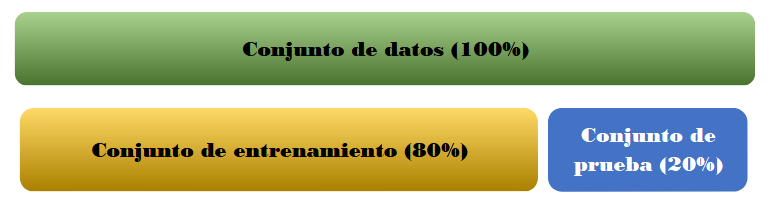
\includegraphics[width=12cm, height=4cm ]{Imagenes/ParticionDEdatos.PNG }
        \caption{Partición del dataset}
        \label{fig:parti}
    \end{figure}

\section{Partición del dataset}



